\documentclass[11pt,twoside]{article}

\usepackage{amssymb}
\usepackage{amsmath}
\usepackage{latexsym}
\usepackage{color}
\usepackage{graphics}
\usepackage{xspace}
\usepackage{amsmath,amsthm,amssymb,graphicx,mathtools,tikz,hyperref}
\usetikzlibrary{automata,positioning}

\newcommand\proofs[1]{\begin{proof}#1\end{proof}}


% Commands for special characters
\newcommand{\mybackslash}{\char'134}
\newcommand{\myleftbracket}{\char'173}
\newcommand{\myrightbracket}{\char'175}
\newcommand{\mypercent}{\char'045}
\newcommand{\myunderscore}{\char'137}

% The 'ifthen' package supports Boolean flags
\usepackage{ifthen}
% The 'solutions' flag determines whether this is the original handout
%    or a solution
\newboolean{solutions}
\setboolean{solutions}{False}  % Default is original handout

% Uncomment the next line before starting on the solutions
\setboolean{solutions}{True}

\newcommand{\coursenumber}{CS 4124}
\newcommand{\coursetitle}{Theory of Computation}
\newcommand{\docdate}{January 11, 2024}
\newcommand{\duedate}{February 2, 2024}
\newcommand{\homeworknumber}{1}

% The document title depends on whether these are solutions
\ifthenelse{\boolean{solutions}}{% Then
\newcommand{\doctitle}{Solutions to Homework Assignment \homeworknumber}
}{% Else
\newcommand{\doctitle}{Homework Assignment \homeworknumber}
}

% The document date depends on whether these are solutions
\ifthenelse{\boolean{solutions}}{% Then
\renewcommand{\docdate}{\duedate}
}{% Else
}

% If you are the author, so put your name here
\renewcommand{\author}{Collin McDevitt}

\pagestyle{myheadings}
\markboth{\hfill\doctitle\hfill\docdate}{\docdate\hfill\doctitle\hfill}

\addtolength{\textwidth}{1.00in}
\addtolength{\textheight}{1.00in}
\addtolength{\evensidemargin}{-1.00in}
\addtolength{\oddsidemargin}{-0.00in}
\addtolength{\topmargin}{-.50in}
\setlength{\footskip}{0pt}

\newcommand{\polyreduce}{\leq_{\mathrm{P}}}

\newcounter{problem}
\setcounter{problem}{0}
\newcommand{\problem}[1]{%
\refstepcounter{problem}\noindent\textbf{[#1] \arabic{problem}.}}

\newcommand{\solution}{\bigskip\hrule\bigskip}
\newcommand{\problembreak}{\bigskip\hrule\bigskip}

\renewcommand{\theenumi}{\textbf{\Alph{enumi}}}
\renewcommand{\theenumii}{\textbf{\roman{enumii}}}

\newcommand{\emptysequence}{\Lambda}
\newcommand{\emptystring}{\epsilon}

% Pseudocode comment symbol
\newcommand{\comment}{\textbf{//}\ \ }

% Pseudocode line numbering
\newcounter{pseudocode}
\newcommand{\firstline}{\setcounter{pseudocode}{0}\linenumber}
\newcommand{\linenumber}{\refstepcounter{pseudocode}\thepseudocode}
\newcommand{\pseudoindent}{\hspace*{26pt}}

\newcommand{\nil}{\mbox{\textsc{nil}}}

% Mathematical symbols
\newcommand{\grid}{\mathcal{G}}  % Grid graph
\newcommand{\integers}{\mathbb{Z}}  % Integers
\newcommand{\Zplus}{\mathbb{Z}^+}  % Positive integers
\newcommand{\naturals}{\mathbb{N}}  % Natural numbers
\newcommand{\reals}{\mathbb{R}}  % Real numbers

% Probability
\newcommand{\expect}[1]{\mathbf{E}\left[#1\right]}
\newcommand{\prob}[1]{\mathrm{Pr}\left[#1\right]}
\newcommand{\var}[1]{\mathrm{Var}\left[#1\right]}

% Logic
\newcommand{\NOT}[1]{\neg #1}
\newcommand{\AND}{\wedge}
\newcommand{\OR}{\vee}
\newcommand{\clause}[1]{\left(#1\right)}

\newlength{\problemoffset}
\setlength{\problemoffset}{0.5in}

% Decision problem macro
% A command for formatting decision problems a la Garey and Johnson
\newcommand{\decision}[3]{%     \decision{NAME}{INSTANCE}{QUESTION}
\begin{list}{}{
\setlength{\leftmargin}{\problemoffset}
\setlength{\rightmargin}{\problemoffset}
\setlength{\parsep}{0pt}
\setlength{\itemsep}{2pt}
\setlength{\topsep}{\itemsep}
\setlength{\partopsep}{\itemsep}
}
\item
{\textsc{#1}}
\item
{INSTANCE: #2}
\item
{QUESTION: #3}
\end{list}
}

% Optimization problem macro
\newcommand{\optimization}[3]{%  \optimization{NAME}{INSTANCE}{SOLUTION}
\begin{list}{}{
\setlength{\leftmargin}{\problemoffset}
\setlength{\rightmargin}{\problemoffset}
\setlength{\parsep}{0pt}
\setlength{\itemsep}{2pt}
\setlength{\topsep}{\itemsep}
\setlength{\partopsep}{\itemsep}
}
\item
{\rule{0pt}{14pt}\textsc{#1}}
\item
{INSTANCE: #2}
\item
{SOLUTION: #3}
\end{list}
}

\newcommand{\reaches}{\leadsto}

% Table layout
\newcommand{\toprule}{\rule[11pt]{0pt}{2pt}}
\newcommand{\bottomrule}{\rule[-6pt]{0pt}{0pt}}
\newenvironment{raggedpars}[1][2.0in]{%
\begin{minipage}[t]{#1}\raggedright\toprule}%
{\bottomrule\end{minipage}}

% Dynamic programming macros
\newlength{\arrowwidth}
\setbox3=\hbox{$\nwarrow$}
\setlength{\arrowwidth}{\wd3}
\newcommand{\optnwarrow}[1]{\if1#1\nwarrow%
\else\rule{\arrowwidth}{0pt}\fi}
\newcommand{\optuparrow}[1]{\if1#1\uparrow%
\else\rule{\arrowwidth}{0pt}\fi}
\newcommand{\optleftarrow}[1]{\if1#1\leftarrow%
\else\rule{\arrowwidth}{0pt}\fi}
% Use \tablebox to specify any combination of arrows, plus the value
\newcommand{\tablebox}[4]{%
\setlength{\arraycolsep}{0.0pt}%
\begin{array}{cc}%
\optnwarrow{#1} & \optuparrow{#2} \\%
\optleftarrow{#3} & #4%
\end{array}%
}
% Use \tableboxred to specify any combination of arrows, plus the value
% The value will be red; arrows are made red if 2 used instead of 1
\newcommand{\optnwarrowred}[1]{\if1#1\nwarrow%
\else\if2#1\textcolor{red}{\nwarrow}\else\rule{\arrowwidth}{0pt}\fi\fi}
\newcommand{\optuparrowred}[1]{\if1#1\uparrow%
\else\if2#1\textcolor{red}{\uparrow}\else\rule{\arrowwidth}{0pt}\fi\fi}
\newcommand{\optleftarrowred}[1]{\if1#1\leftarrow%
\else\if2#1\textcolor{red}{\leftarrow}\else\rule{\arrowwidth}{0pt}\fi\fi}
\newcommand{\tableboxred}[4]{%
\setlength{\arraycolsep}{0.0pt}%
\begin{array}{cc}%
\optnwarrowred{#1} &%
\optuparrowred{#2} \\%
\optleftarrowred{#3} &%
\textcolor{red}{#4}%
\end{array}%
}

% Allow really sloppy paragraphs that do not generate overfull or
%    underfull hbox's
\newenvironment{SLOPPY}{\begin{sloppypar}\hbadness=10000}{\end{sloppypar}}

% Definitions for this homework
\newcommand{\extent}[1]{\mathrm{extent}(#1)}
\newcommand{\opt}[2]{\mbox{\textsc{opt}}(#1,#2)}
\newcommand{\gap}{\mbox{\texttt{-}}}
\newcommand{\rewriterule}[2]{#1\to #2}
\newcommand{\rewrites}[2][]{\mathop{\Longrightarrow}\limits_{#1}^{#2}}
\newcommand{\reduces}{\leq}
\newcommand{\polyreduces}{\leq_P}
\newcommand{\mathsc}[1]{\mbox{\normalfont\textsc{#1}}}
\newcommand{\NP}{\mathcal{NP}}
\renewcommand{\P}{\mathcal{P}}
\newcommand{\describes}{\vdash}

\begin{document}

\thispagestyle{empty}

\begin{center}
    \begin{tabular}{lcr}
        \multicolumn{3}{c}{\Large\textbf{\coursenumber}}
        \\[0.04in]
        \multicolumn{3}{c}{\Large\textbf{\doctitle}}
        % If these are solutions, then include the author's (student's) name
        \ifthenelse{\boolean{solutions}}{% Then
        \\[0.04in]\multicolumn{3}{c}{\large\textbf{\author}}
        }{} % Else omit
        % If these are solutions, then the date is the due date
        \ifthenelse{\boolean{solutions}}{% Then
        \\[0.10in]\multicolumn{3}{c}{\duedate}
        }{% Else, put given and due dates
        \\[0.10in]
            \textbf{Given:} \docdate
         & \hspace*{1.0in} &
            \textbf{Due:} \duedate
        }
    \end{tabular}
\end{center}

% If these are solutions, then we do not include the directions
\ifthenelse{\boolean{solutions}}{} % No directions
{
    % Original document includes directions
    \begingroup % This allows an argument that contains multiple paragraphs
    \paragraph{General directions.}
    The point value of each problem is shown in [ ].
    Each solution must include all details and
    an explanation of why the given solution is correct.
    \textbf{\textcolor{red}{In particular,
            write complete sentences.
            A correct answer without an explanation is worth no credit.}}
    The completed assignment must be submitted on Canvas as a PDF by 5:00 PM
    on \duedate.
    \textbf{No late homework will be accepted.}

    \paragraph{Digital preparation of your solutions is mandatory.
        This includes digital preparation of any drawings; see syllabus
        concerning neat drawings included in \LaTeX\ solutions.}
    \textbf{Use of \LaTeX\ is required.
        Also,
        please include your name.}

    \paragraph{Use of \LaTeX\ (required).}
    \begin{itemize}
        \item Retrieve this \LaTeX\ source file,
              named
              \texttt{homework\homeworknumber.tex},
              from the course web site.
        \item Rename the file
              \textit{$<$Your VT PID$>$}\texttt{{\myunderscore}solvehw\homeworknumber.tex},
              For example,
              for the instructor,
              the file name would be
              \texttt{heath{\myunderscore}solvehw\homeworknumber.tex}.

        \item
              Use a \textbf{text editor}
              (such as \texttt{vi}, \texttt{emacs}, or \texttt{pico})
              to accomplish the next three steps.
              Alternately,
              use Overleaf as your \LaTeX\ platform.

        \item
              Uncomment the line

              \texttt{{\mypercent}
                  {\mybackslash}setboolean{\myleftbracket}solutions{\myrightbracket}%
              {\myleftbracket}True{\myrightbracket}}

              in the document preamble by deleting the \texttt{\mypercent}.

        \item
              Find the line

              \texttt{{\mybackslash}renewcommand%
              {\myleftbracket}{\mybackslash}author{\myrightbracket}%
              {\myleftbracket}Lenwood S. Heath{\myrightbracket}}

              and replace the instructor's name with your name.

        \item
              Enter your solutions where you find
              the \LaTeX\ comments

              \texttt{{\mypercent} PUT YOUR SOLUTION HERE}

        \item
              Generate a PDF and turn it in on Canvas by 5:00 PM on \duedate.
    \end{itemize}
    \endgroup

    \problembreak

    \newpage

}

\problem{25}
{\bfseries
Textbook Problem 5 in B.1
on Page 520.

Prove Lemma A.4:
For all alphabets $\Sigma$
and all languages $L\subseteq\Sigma^\star$,
the equivalence relation
$\equiv_L$ is right-invariant.

The lemma
and the definition of the equivalence relation are on Page 505.
}

\solution

\begin{proof}
    Let $\Sigma$ be an alphabet and $L\subseteq \Sigma^{*}$ and $\equiv_L$ be
    an equivalence relation as defined by (A.3). Let $x,y,z,w \in \Sigma^{*}$ and $x\equiv_L y$ then we have $xz,yz\in L$ as $zw\in \Sigma^{*}$ we have $xzw,yzw\in L$ which implies $xz\equiv_L yz$.
\end{proof}

\problembreak

\problem{25}
{\bfseries
Textbook Problem 3(c) in B.2
on Page 522.

Design an FA $M$,
with alphabet $\Sigma=\{0,1\}$,
that recognizes
(c) the set of all strings that contain the string $011$,
in that order,
but not necessarily consecutively.

Be certain you understand the set (language) of $M$
before you start designing.
Constructing some examples of strings both in $L(M)$ and not in $L(M)$
can be helpful.

You may use an algebraic specification
or a transition diagram (labeled directed graph) specification
to present your design for $M$.
Be certain to explain why your design works.
}

\solution

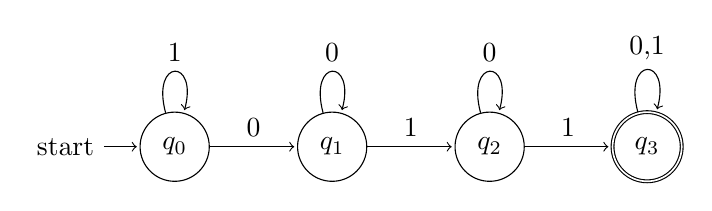
\begin{tikzpicture}[shorten >=1pt,node distance=2cm,on grid,auto]
    \node[state,initial] (q_0)   {$q_0$};
    \node[state] (q_1) [right=of q_0] {$q_1$};
    \node[state] (q_2) [right=of q_1] {$q_2$};
    \node[state,accepting](q_3) [right=of q_2] {$q_3$};
    \path[->]
    (q_0) edge  node {0} (q_1)
    edge [loop above] node {1} ()
    (q_1) edge  node  {1} (q_2)
    edge [loop above] node {0} ()
    (q_2) edge [loop above] node {0} ()
    (q_2) edge  node  {1} (q_3)
    (q_3) edge [loop above] node {0,1} ();

\end{tikzpicture}

This design for a \textbf{FA} works as reading through the input string we have it only enters state $q_1$ if it has read $0$ and will loop otherwise. Then for each of the next states $q_1,q_2$ they will loop if they receive a $0$ otherwise they will go to $q_2$ and $q_3$ respectively. $q_3$ is an accepting state and will loop for any input which ensures that the string only need to contain $011$ not end in that.


\problembreak

\problem{25}
{\bfseries
Consider the OA $M_4$ in Figure 3.4
on Page 60.
Give a complete and careful algebraic specification
\begin{eqnarray*}
    M_4
    & = &
    (Q,\Sigma,\delta,q_0,F)
\end{eqnarray*}
for $M_4$.
}

\solution

% PUT YOUR SOLUTION HERE

\problembreak

\problem{25}
{\bfseries
Textbook Problem 7(c) in B.2
on Pages 522 and 523.

Use a (fooling set)-plus-(Continuation Lemma) argument to prove
that the following language is \textit{not} Regular:
\begin{eqnarray*}
    L_5
    & = &
    \{a^ib^jc^k \mid i=j \mbox{\normalfont\ \textsc{or}\ } j=k\}.
\end{eqnarray*}
Your argument will be a proof by contradiction.

The Continuation Lemma is Lemma 3.2 on Page 57,
while the fooling set kind of argument is first utilized
on Pages 76 and 77.
}

\solution

% PUT YOUR SOLUTION HERE

\problembreak

\end{document}